%----------------------------------------------------------------------------------------
%    PACKAGES AND THEMES
%----------------------------------------------------------------------------------------

\documentclass[aspectratio=169,xcolor=dvipsnames]{beamer}
\usetheme{SimplePlus}

\usepackage{hyperref}
\usepackage{graphicx} % Allows including images
\usepackage{booktabs} % Allows the use of \toprule, \midrule and \bottomrule in tables
\usepackage{array} % Allows >{\centering\arraybackslash} in tabular

%----------------------------------------------------------------------------------------
%    TITLE PAGE
%----------------------------------------------------------------------------------------

\title{Stochastic Optimal Control Matching}
\subtitle{Carles Domingo-Enrich, Jiequn Han, Brandon Amos, Joan Bruna, Ricky T. Q. Chen}

\author{Thomas Mousseau}

% \institute
% {
%     Department of Computer Science and Information Engineering \\
%     National Taiwan University % Your institution for the title page
% }
\date{\today} % Date, can be changed to a custom date

%----------------------------------------------------------------------------------------
%    PRESENTATION SLIDES
%----------------------------------------------------------------------------------------

\begin{document}

\begin{frame}
    % Print the title page as the first slide
    \titlepage
\end{frame}

\begin{frame}{Overview}
    % Throughout your presentation, if you choose to use \section{} and \subsection{} commands, these will automatically be printed on this slide as an overview of your presentation
    \tableofcontents
\end{frame}

%------------------------------------------------
\section{Setup and Preliminaries}

%TODO: J'aimerais beaucoup glisser les Continuous Normalizing Flows a.k.a Neural ODE avant DDPM et le reste puisque c'est vrm un paper essential a research field
\begin{frame}{Neural ODE: Continuous Normalizing Flows}

    \begin{block}{Continuous Normalizing Flows (CNF)}
        CNFs model complex distributions by transforming a simple distribution (e.g., Gaussian) through a continuous-time ODE. The transformation is defined by a neural network that learns the dynamics of the flow.
    \end{block}

    PAS COMPLETE
    
    \vspace{0.3cm}
    
    \begin{alertblock}{Key Idea}
        Instead of discrete steps, CNFs use a continuous-time approach to model the evolution of the distribution, allowing for more flexible and expressive transformations.
    \end{alertblock}
\end{frame}

\begin{frame}{Evolution of Generative Models}
    \begin{center}
        \begin{minipage}{0.9\textwidth}
            \vspace{0.3cm}
            
            \small
            \begin{tabular}{@{}l@{\hspace{0.8cm}}p{0.75\textwidth}@{}}
                \textbf{2020} & \textbf{DDPM:} Denoising Diffusion Probabilistic Models interpret generation as reversing a discrete noise-adding process, learning to denoise at each step. They produced high-quality samples but required thousands of slow sampling steps. \\[0.4cm]
                
                \textbf{2021} & \textbf{Score-based Models:} Score-based generative models extended diffusion to continuous-time SDEs, learning the score function ($\nabla_x \log p_t(x)$) to reverse a stochastic diffusion process. This unified diffusion with stochastic control, allowed probability flow ODEs, and sped up sampling. \\[0.4cm]
                
                \textbf{2023} & \textbf{Flow Matching:} Flow matching views generation as learning a deterministic ODE vector field that directly transports a simple distribution (e.g., Gaussian) to data. This removed stochasticity and significantly improved efficiency compared to diffusion/score methods. \\[0.4cm]
            \end{tabular}
            
            \vspace{0.3cm}
        \end{minipage}
    \end{center}
\end{frame}

\begin{frame}{What is a Stochastic Control Problem?}
    A stochastic control problem involves finding an optimal control policy to steer a dynamical system under uncertainty.
    
    \vspace{0.3cm}
    
    \begin{block}{Key Components}
        \begin{itemize}
            \item \textbf{State Process:} $X_t \in \mathbb{R}^d$ (position in state space at time $t$)
            \item \textbf{Control Process:} $u_t \in \mathbb{R}^d$ (action/decision at time $t$)
            \item \textbf{Noise Process:} $W_t$ (random disturbances, typically Brownian motion)
        \end{itemize}
    \end{block}
    
    \begin{columns}[t]
        \column{0.45\textwidth}
        \begin{alertblock}{Dynamics (SDE)}
            \vspace{-0.1cm}
            \begin{equation}
            dX_t = f(X_t, u_t, t) dt + g(X_t, t) dW_t
            \end{equation}
            \vspace{-0.2cm}
        \end{alertblock}
        
        \column{0.52\textwidth}
        \begin{alertblock}{Cost Function}
            \vspace{-0.1cm}
            \begin{equation}
            J(u) = \mathbb{E}\left[\int_0^T L(X_t, u_t, t) dt + \Phi(X_T)\right]
            \end{equation}
            \vspace{-0.2cm}
        \end{alertblock}
    \end{columns}
\end{frame}

\begin{frame}{The Goal: Finding Optimal Control}
    \begin{block}{Optimal Control $u^*$}
        Find the control policy $u^*$ that minimizes the expected cost: $u^* = \arg\min_u J(u)$
    \end{block}
    
    \vspace{0.3cm}
    
    \begin{block}{Classical Approaches}
        \begin{itemize}
            \item \textbf{Hamilton-Jacobi-Bellman (HJB) equation:} Partial differential equation approach
            % \item \textbf{Pontryagin's Maximum Principle:} Necessary conditions for optimality
            \item \textbf{Dynamic Programming:} Discrete-time recursive approach
        \end{itemize}
    \end{block}
    
    \vspace{0.3cm}
    
    \begin{alertblock}{Challenge}
        These classical methods become computationally intractable in high dimensions due to the \textit{curse of dimensionality}.
    \end{alertblock}
\end{frame}

%TODO: A voir si je veux expliquer ce qu'est une Adjoint Method?!?!??!?!?!?

%TODO: A voir encore si je ne veux pas faire un lien avec RL ou meme directement presente la HJB et demontrer que ls Jacobienne devient difficulement calculate (prix computationnel trop eleve) a plusieurs dimensions
%! For continuous-time problems with low-dimensional state spaces, the standard approach to learn
%! the optimal control is to solve the Hamilton-Jacobi-Bellman (HJB) partial differential equation
%! (PDE) by gridding the space and using classical numerical methods. For high-dimensional problems,
%! a large number of works parameterize the control using a neural network and train it applying a
%! stochastic optimization algorithm on a loss function. These methods are known as Iterative Diffusion
%! Optimization (IDO) techniques [59] (see Subsec. 2.2).

%------------------------------------------------

%------------------------------------------------
% \section{Setup and preliminaries}
%------------------------------------------------

%------------------------------------------------
\section{Stochastic Optimal Control Matching}

\begin{frame}{Reasons behind SOCM (1/2)}
    Many fundamental tasks in machine learning can be naturally cast as stochastic optimal control problems, highlighting the importance of efficient SOC methods.
    
    \vspace{0.4cm}
    
    \begin{block}{Key ML Applications of SOC}
        \begin{itemize}
            \item \textbf{Reward fine-tuning of diffusion and flow models:} Optimizing generation quality using reward signals
            
            \vspace{0.2cm}
            
            \item \textbf{Conditional sampling on diffusion and flow models:} Steering generation towards specific conditions or constraints
            
            \vspace{0.2cm}
            
            \item \textbf{Sampling from unnormalized densities:} Efficiently drawing samples from complex, intractable distributions
            
            \vspace{0.2cm}
            
            \item \textbf{Importance sampling of rare events in SDEs:} Computing probabilities of low-probability but critical events
        \end{itemize}
    \end{block}
    
    \vspace{0.3cm}
    
    \begin{alertblock}{Key Insight}
        The prevalence of SOC formulations in modern ML motivates the need for more efficient and stable solving methods.
    \end{alertblock}
\end{frame}

\begin{frame}{Reasons behind SOCM (2/2)}
    Current SOC methods suffer from optimization challenges that limit their effectiveness.
    
    \vspace{0.3cm}
    
    \begin{columns}[t]
        \column{0.48\textwidth}
        \begin{alertblock}{Current SOC Methods}
            \begin{itemize}
                \item Use \textbf{adjoint methods} (like CNFs)
                \item Yield \textbf{non-convex} function landscapes
                \item Difficult optimization with local minima
                \item Unstable training dynamics
            \end{itemize}
        \end{alertblock}
        
        \column{0.48\textwidth}
        \begin{block}{Diffusion Models Success}
            \begin{itemize}
                \item Use \textbf{least-squares loss}
                \item Create \textbf{convex} functional landscapes
                \item Stable and reliable optimization
                \item Excellent empirical performance
            \end{itemize}
        \end{block}
    \end{columns}
    
    \vspace{0.4cm}
    
    \begin{block}{SOCM's Innovation}
        \textbf{Goal:} Develop least-squares loss formulations for SOC problems, combining the expressiveness of stochastic control with the optimization stability of diffusion models.
    \end{block}
\end{frame}


\begin{frame}{SOCM in Context: Optimization Landscapes}
    \vspace{0.5cm}
    \begin{table}
        \centering
        \begin{tabular}{>{\centering\arraybackslash}p{0.25\textwidth}>{\centering\arraybackslash}p{0.35\textwidth}>{\centering\arraybackslash}p{0.35\textwidth}}
            \toprule
            \textbf{Task} & \textbf{Non-convex} & \textbf{Least Squares} \\
            \midrule
            Generative Modeling & Maximum Likelihood CNFs & Diffusion models and Flow Matching \\
            Stochastic Optimal Control & Adjoint Methods & \textcolor{red}{\textbf{Stochastic Optimal Control Matching}} \\
            \bottomrule
        \end{tabular}
    \end{table}
\end{frame}

\begin{frame}{Introducing Stochastic Optimal Control Matching}
    SOCM offers a more principled, stable, and accurate way to learn generative dynamics by blending stochastic control theory with modern matching-based generative modeling.
    
    \vspace{0.4cm}
    
    \begin{block}{Key Novel Contributions}
        \begin{enumerate}
            \item \textbf{Controlled Stochastic Process:} Views the generation process as a controlled stochastic process bridging a simple distribution to data.
            
            \vspace{0.2cm}
            
            \item \textbf{Least-Squares Matching:} Learning the control via least-squares matching, a stable and convex regression objective.
            
            \vspace{0.2cm}
            
            \item \textbf{Joint Optimization:} Optimizing control and variance-reducing reparameterization matrices simultaneously, for efficient learning.
            
            \vspace{0.2cm}
            
            \item \textbf{Path-wise Reparameterization:} Introducing a path-wise reparameterization trick, boosting gradient estimation quality.
        \end{enumerate}
    \end{block}
\end{frame}


\begin{frame}{The SOCM Framework}
    \small
    \begin{block}{SOCM Loss Function}
        The Stochastic Optimal Control Matching objective is defined as:
        \begin{equation}
        \mathcal{L}_{SOCM}(u, M) := \mathbb{E}\left[\frac{1}{T}\int_0^T \|u(X^v_t, t) - w(t, v, X^v, B, M_t)\|^2 dt \times \alpha(v, X^v, B)\right]
        \end{equation}
    \end{block}

    \begin{block}{Where:}
        \begin{itemize}
            \item $X^v$ is the process controlled by $v$: 
            \begin{equation}
            dX^v_t = (b(X^v_t, t) + \sigma(t)v(X^v_t, t)) dt + \sqrt{\lambda}\sigma(t) dB_t
            \end{equation}
            with $X^v_0 \sim p_0$
            \item $u(X^v_t, t)$ is the control policy being learned
            \item $w(t, v, X^v, B, M_t)$ is the target matching function
            \item $\alpha(v, X^v, B)$ is a weighting function
        \end{itemize}
    \end{block}
\end{frame}

\begin{frame}{SOCM Algorithm}
    \begin{figure}
        \centering
        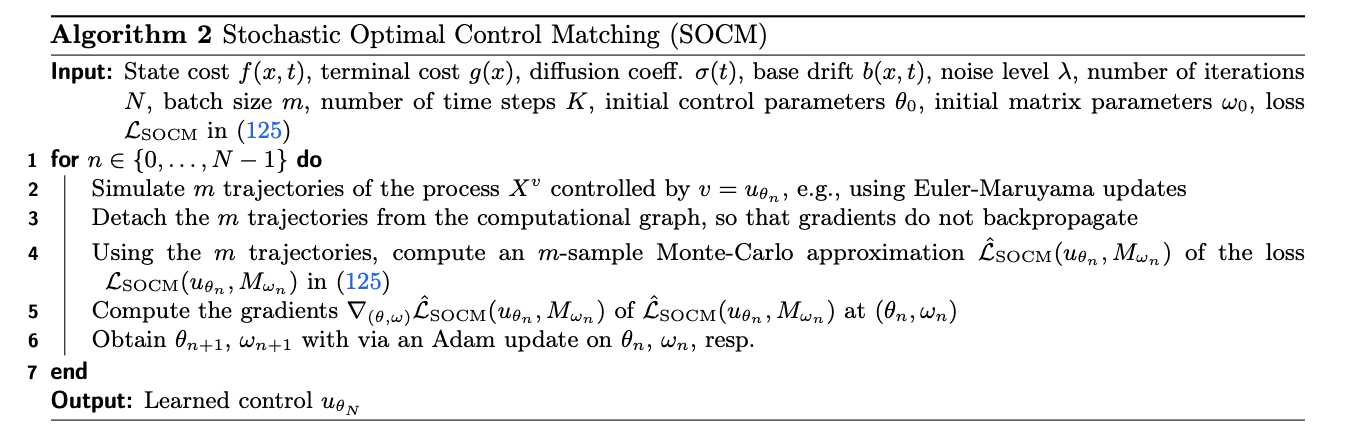
\includegraphics[width=0.95\textwidth]{figures/SOCM_algo.png}
        \caption{Stochastic Optimal Control Matching (SOCM) Algorithm}
    \end{figure}
\end{frame}

\begin{frame}{Experimental Results (1/2)}
    \begin{figure}
        \centering
        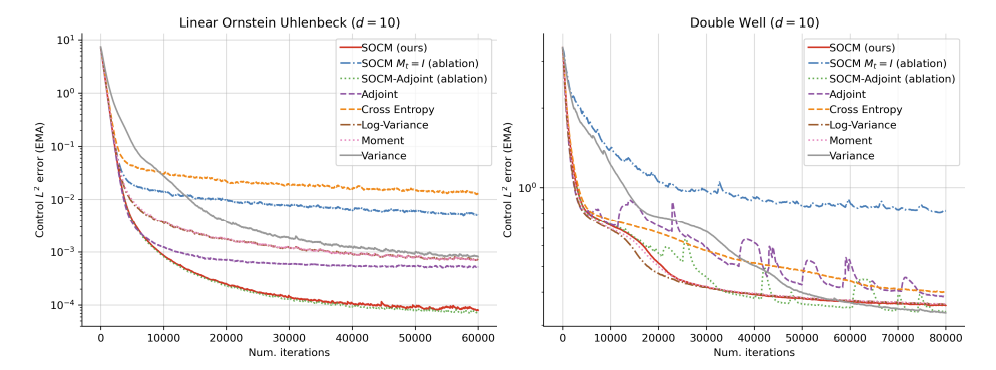
\includegraphics[width=0.95\textwidth]{figures/plots_1.png}
    \end{figure}
\end{frame}

\begin{frame}{Experimental Results (2/2)}
    \begin{figure}
        \centering
        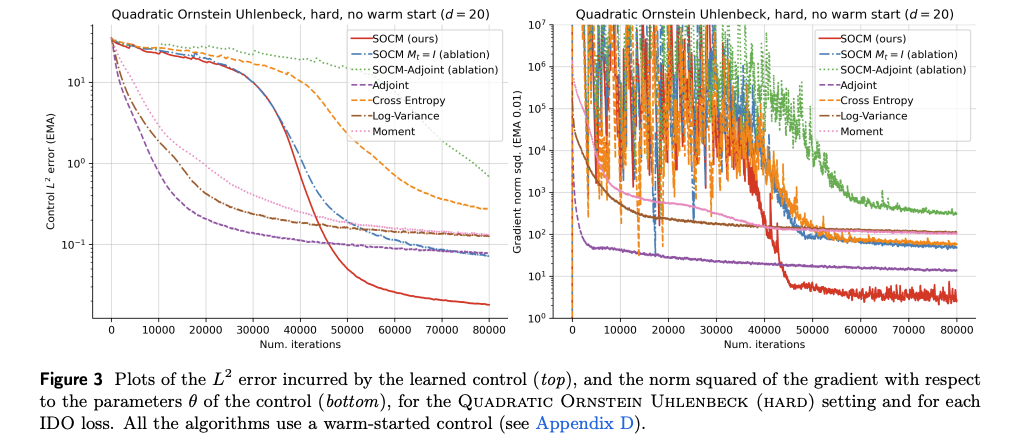
\includegraphics[width=0.95\textwidth]{figures/plots_2.png}
    \end{figure}
\end{frame}
%------------------------------------------------

%------------------------------------------------
\section{Experiments and results}
%------------------------------------------------

%------------------------------------------------
\section{Conclusion}

%! so many links to do with RL and Monte Carlo Markov Chains which representent discretized differential equations
%------------------------------------------------


% \begin{frame}{Bullet Points}
%     \begin{itemize}
%         \item Lorem ipsum dolor sit amet, consectetur adipiscing elit
%         \item Aliquam blandit faucibus nisi, sit amet dapibus enim tempus eu
%         \item Nulla commodo, erat quis gravida posuere, elit lacus lobortis est, quis porttitor odio mauris at libero
%         \item Nam cursus est eget velit posuere pellentesque
%         \item Vestibulum faucibus velit a augue condimentum quis convallis nulla gravida
%     \end{itemize}
% \end{frame}

%------------------------------------------------

\begin{frame}{Blocks of Highlighted Text}
    In this slide, some important text will be \alert{highlighted} because it's important. Please, don't abuse it.

    \begin{block}{Block}
        Sample text
    \end{block}

    \begin{alertblock}{Alertblock}
        Sample text in red box
    \end{alertblock}

    \begin{examples}
        Sample text in green box. The title of the block is ``Examples".
    \end{examples}
\end{frame}

%------------------------------------------------

\begin{frame}{Multiple Columns}
    \begin{columns}[c] % The "c" option specifies centered vertical alignment while the "t" option is used for top vertical alignment

        \column{.45\textwidth} % Left column and width
        \textbf{Heading}
        \begin{enumerate}
            \item Statement
            \item Explanation
            \item Example
        \end{enumerate}

        \column{.45\textwidth} % Right column and width
        Lorem ipsum dolor sit amet, consectetur adipiscing elit. Integer lectus nisl, ultricies in feugiat rutrum, porttitor sit amet augue. Aliquam ut tortor mauris. Sed volutpat ante purus, quis accumsan dolor.

    \end{columns}
\end{frame}

%------------------------------------------------

\begin{frame}{Table}
    \begin{table}
        \begin{tabular}{l l l}
            \toprule
            \textbf{Treatments} & \textbf{Response 1} & \textbf{Response 2} \\
            \midrule
            Treatment 1         & 0.0003262           & 0.562               \\
            Treatment 2         & 0.0015681           & 0.910               \\
            Treatment 3         & 0.0009271           & 0.296               \\
            \bottomrule
        \end{tabular}
        \caption{Table caption}
    \end{table}
\end{frame}

%------------------------------------------------

\begin{frame}{Theorem}
    \begin{theorem}[Mass--energy equivalence]
        $E = mc^2$
    \end{theorem}
\end{frame}

%------------------------------------------------

\begin{frame}{Figure}
    Uncomment the code on this slide to include your own image from the same directory as the template .TeX file.
    %\begin{figure}
    %\includegraphics[width=0.8\linewidth]{test}
    %\end{figure}
\end{frame}

%------------------------------------------------

\begin{frame}[fragile] % Need to use the fragile option when verbatim is used in the slide
    \frametitle{Citation}
    An example of the \verb|\cite| command to cite within the presentation:\\~

    This statement requires citation \cite{p1}.
\end{frame}

%------------------------------------------------

\begin{frame}{References}
    \footnotesize
    \bibliography{reference.bib}
    \bibliographystyle{apalike}
\end{frame}

%------------------------------------------------

\end{document}